\documentclass{beamer}

%\usepackage[utf8x]{inputenc}
\usepackage{textcomp}

\definecolor{OSUdkbrn}{RGB}{104,80,64}
\definecolor{OSUmedbrn}{RGB}{176,96,16}
\definecolor{OSUltbrn}{RGB}{224,195,152}
% from: http://oregonstate.edu/brand/color-palette


\usepackage[backend=biber,citestyle=authoryear,bibstyle=authoryear,maxbibnames=10]{biblatex}
\addbibresource{../report/VCPbibliography.bib}

\mode<presentation>
{
	\usetheme{CambridgeUS}
	\setbeamercovered{transparent}
	\setbeamertemplate{footline}[page number]{}
	\setbeamercolor{palette tertiary}{fg=white, bg=OSUdkbrn}
	\setbeamercolor{title}{fg=OSUdkbrn}
	\setbeamercolor{frametitle}{fg=OSUdkbrn}
	\setbeamertemplate{itemize items}[square]
	\setbeamercolor*{item}{fg=OSUdkbrn}
}

\title{Variable Circular Plots: Station Placement and the Independence Assumption}
\subtitle{Master's Research Project}
\author{Matt Edwards\\ Advisor: Claudio Fuentes}
\date{June 11, 2014}

\begin{document}
\begin{frame}
	\titlepage
\end{frame}

%\begin{frame}
%	\frametitle{Outline}
%	\tableofcontents
%\end{frame}

% -------------------------------- INTRODUCTION --------------------------------------------------
\section{Introduction}

\begin{frame}{Distance Sampling}
	\begin{itemize}
	\item Population Density Estimation
	\item[]
	\item Used often in Ecological Sciences
	\item[]
	\item Began with roadside surveys in early 1900s
	\item[]
	\item Theory developed through mid-1900s
	
	\end{itemize}
\end{frame}

\begin{frame}{Distance Sampling: History}
	\begin{itemize}
	\item Emlen---1971
	\item Ramsey, Scott---1979, 1980 Papers
	\item Burnham, Anderson, and Jeffrey L. Laake---1980 Monograph
	\item Buckland et. al. 1993, 2001---text
	\item Continued Development into 2000s
	\begin{itemize}
	\item Combined with Mark-Recapture Methods
	\item Extended for use with underwater acoustics for estimates of krill populations 
	\item Combined with camera traps to estimate populations
	\end{itemize}
	\end{itemize}
\end{frame}

\begin{frame}{Line Vs. Point Transects}
	\begin{itemize}
	\item Line transects are walked
	\begin{itemize}
		\item Distances perpendicular to transect are recorded, as projected on ground
	\end{itemize}
	\item[]
	\item Point transects: observer(s) stand at station, observe everything within 360\textdegree 
		\begin{itemize}
		\item Alternately: Variable Circular Plots (VCP)
		\item Allow ``cooling'' period
		\item Safer for observer
		\item Straight line distance from Observer is recorded, as projected on ground
		\end{itemize}
	\item[]		
	\item Observations can be from visual sightings, auditory clues, or a combination
	\end{itemize}
\end{frame}

\begin{frame}{Detection Curve: $g(r)$}
	\begin{figure}
		\centering
		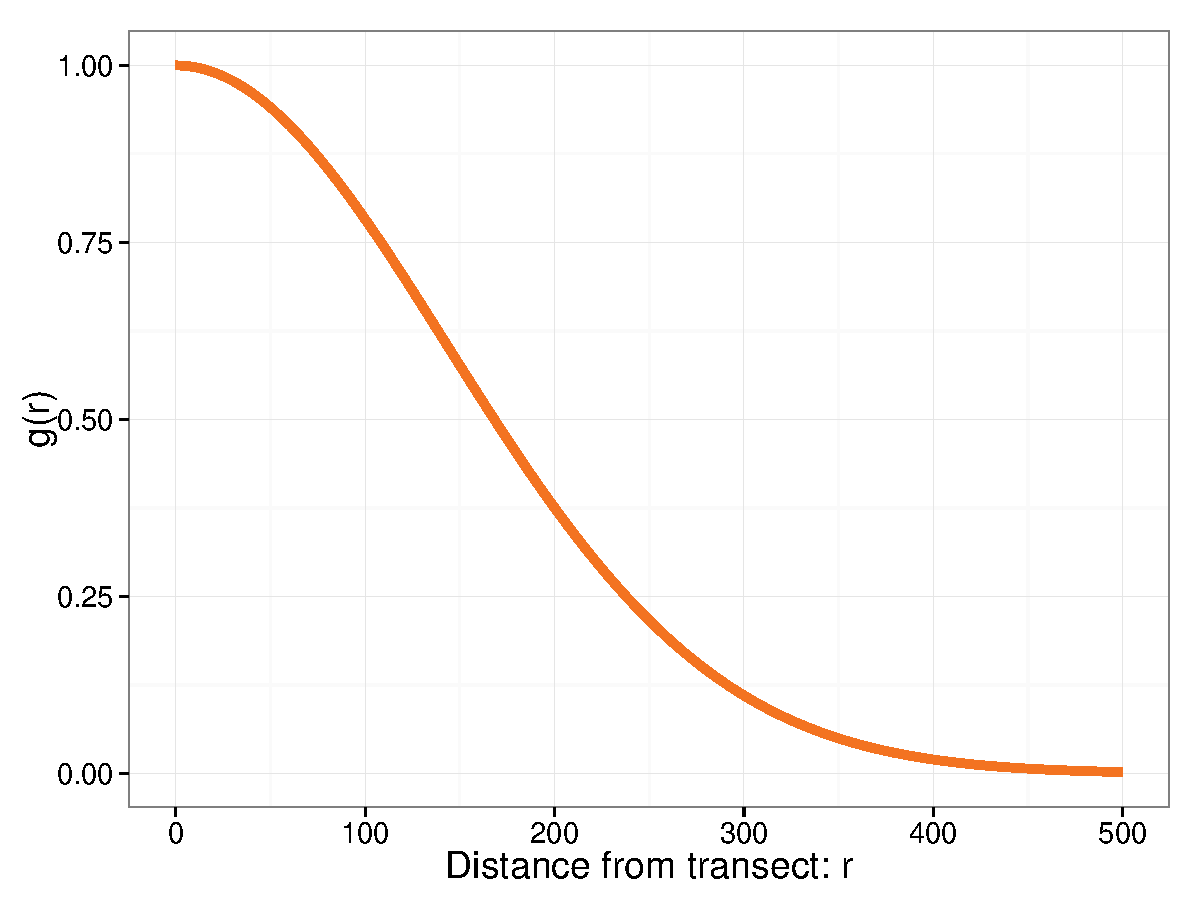
\includegraphics[width=\textwidth,height=0.80\textheight,keepaspectratio=true]{../images/detectionCurve.pdf}
	\end{figure}
	\note{
		\begin{itemize}
		\item Perfect Detectability Near to Observer, dropping off. The ``shoulder''
		\item $g(r)$ = probability of detecting an object, given it is at distance $r$
		\item scaled so $g(0) = 1$
		\end{itemize}
	}
\end{frame}

\begin{frame}{Density Estimation}
	\begin{center}
	$\hat{D}=\dfrac{n}{\mbox{Area}*P(\mbox{observing object}|\mbox{distance }r)}$\\
	\vspace{0.5cm}
	$\hat{D}=\dfrac{n}{\mbox{Area}*g(r)}$
	\end{center}

	\note{
		\begin{itemize}
		\item Much of the difficulty in distance sampling comes from estimating g(r)
		\item For this presentation, the kernel method, a non-parametric method, was used.
		\item in very broad terms, it looks at the average count per VCP and estimates area and probability by averaging over the observed observation distances inside a normal kernel. 
		\end{itemize}
	}
\end{frame}

\begin{frame}{Micronesian Forest Bird Survey: 1982}
\begin{itemize}
\item Engbring, Ramsey \& Wildman (1986)
\item[]
\item Used VCP to survey several bird species in the Micronesian islands
\item[]
\item Each of 5 Islands divided into regions
\item[]
\item Transect randomly placed within region (angle \& starting position selected randomly)
\item[]
\item Stations placed every 150 m along transect
\item[]
\item Additional transects placed 2 km parallel
\end{itemize}

	\note{
	\begin{itemize}
	\item Observers would wait 2 minutes after arrival, then spend 8 minutes observing all they could
	\item Distance and species were noted, as well as foliage and other variables.
	\end{itemize}
	}
\end{frame}

\begin{frame}{Collared Kingfisher Observation Data}

\begin{figure}
	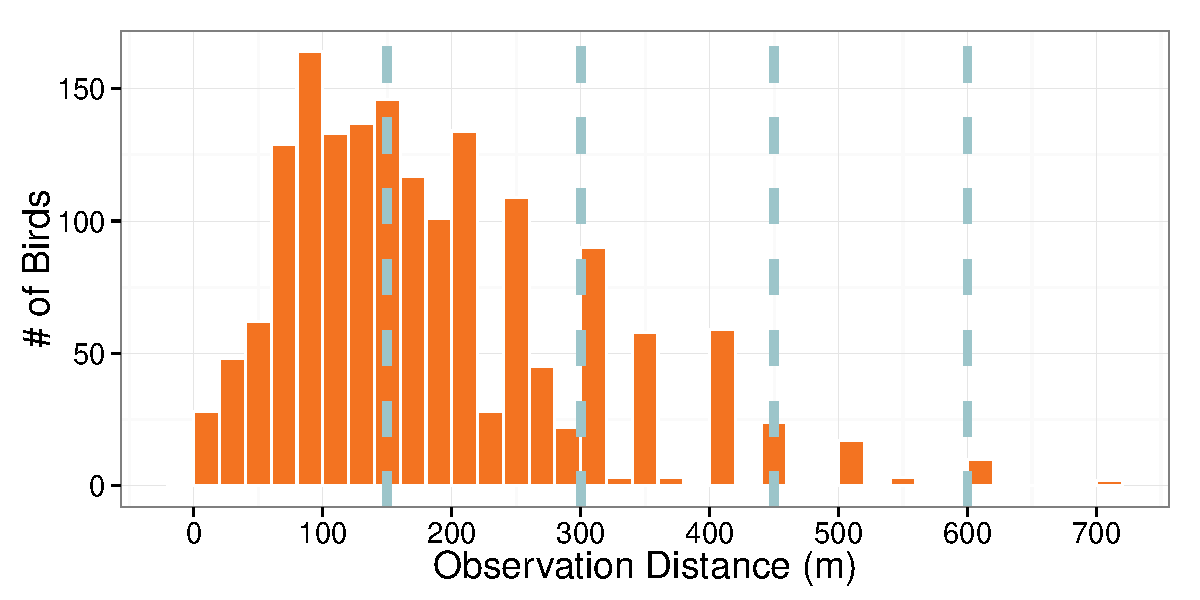
\includegraphics[width=\textwidth]{../images/histogram_dist_20m.pdf}
	\label{fig:82dist}
\end{figure}

	\note{
		\begin{itemize}
		\item Aggregated over two islands, Rota \& Tinan
		\item Aggregated over all observers, 4
		\item Primarily auditory cues, some visual, and some heard-then-seen
		\item Data tell us 3 main things
		\begin{itemize}
			\item Very low bird counts immediately around the station. Some evidence of movement.
			\item Evidence of heaping, the further away from station. More prominent with smaller bins.
			\item Stations places 150 Meters Apart.
		\end{itemize}
		\end{itemize}
	}
\end{frame}

\begin{frame}{Research Question}
Do overlapping observation areas violate any underlying independence assumptions?\\
\vspace{1cm}Will it make a difference in our final population density estimates if a bird is observed from more than one station?
\end{frame}

\begin{frame}{VCP Indepencence}
	\begin{itemize}
	\item \textcite{ramsey1979,buckland1987,thompson2012} discuss assumption that VCPs are randomly placed.
	\begin{itemize}
	\item Implicit, but not explicit, possibility of overlap
	\end{itemize}
	\item[]
	\item \textcite{reynolds1980} state the possibility of observing the same bird from more than one station should be avoided.
	\item[]
	\item \textcite{buckland2001} states ``Transects are normally spaced at a sufficient distance to avoid detecting an object from two neighboring transacts, although this is not usually critical unless sampling a line changes the animal distribution at neighboring, as yet un-sampled lines.''
	\end{itemize}
	
		\note{
			\begin{itemize}
			\item Some Selected Quotes
			\item Literature is divided
			\item Transect layouts, similar to micronesian study, are common
			\item We as scientists need to understand how this might bias our results.
			\end{itemize}
		}
\end{frame}







\begin{frame}{Final Words}
\begin{quote}
``All models are wrong, but some are useful.'' --George E. P. Box
\end{quote}


\end{frame}


\end{document}
